\documentclass[12pt]{article}
\usepackage{graphicx}
\usepackage{float}
\usepackage{caption}
\usepackage{subcaption}
\usepackage{geometry}
\geometry{a4paper, margin=1in}
\usepackage{amsmath, amsfonts, amssymb}
\usepackage{booktabs, array}
\usepackage{fancyhdr}
\usepackage{titlesec}
\usepackage{listings}
\usepackage{xcolor}
\usepackage[hidelinks]{hyperref}
\usepackage{enumitem}
\usepackage{cite}
\usepackage{listings}
\usepackage{subcaption}
\usepackage{url}
\usepackage{hyperref}
\usepackage[T1]{fontenc}
\usepackage[scaled]{beramono} % optional: better monospace font





\lstdefinestyle{pythonstyle}{
    language=Python,
    basicstyle=\linespread{1.1}\ttfamily\footnotesize,
    keywordstyle=\color{blue}\bfseries,
    commentstyle=\color{green!60!black}\itshape,
    stringstyle=\color{red},
    showstringspaces=false,
    breaklines=true,
    frame=single,
    numbers=left,
    numberstyle=\tiny\color{gray},
    tabsize=4,
    backgroundcolor=\color{gray!5},
    xleftmargin=1.5em,
    framexleftmargin=1.5em,
    morekeywords={
        np, cv2, array, linspace, arange, reshape, dtype,
        uint8, float32, float64, int32, int64,
        zeros, ones, eye, mean, median, std, var,
        sum, max, min, clip, concatenate, hstack, vstack,
        imread, imshow, imwrite, cvtColor, COLOR_BGR2GRAY,
        GaussianBlur, filter2D, Sobel, Laplacian,
        bitwise_and, threshold, inRange, findContours,
        moments, boundingRect, rectangle, circle,
        waitKey, destroyAllWindows
    }
}

\lstdefinestyle{cppstyle}{
    language=C++,
    basicstyle=\ttfamily\footnotesize,
    keywordstyle=\color{blue}\bfseries,                 % C++ keywords
    commentstyle=\color{green!60!black}\itshape,        % Comments
    stringstyle=\color{red},                            % Strings
    showstringspaces=false,
    breaklines=true,
    frame=single,
    numbers=left,
    numberstyle=\tiny\color{gray},
    backgroundcolor=\color{gray!5},
    xleftmargin=1.5em,
    framexleftmargin=1.5em,
    morekeywords={
        auto, nullptr, static_cast, dynamic_cast, const_cast, reinterpret_cast,
        cv, Mat, Vec3b, Point, Size, Scalar, Rect, RotatedRect, Range,
        VideoCapture, imread, imshow, imwrite, resize, cvtColor, GaussianBlur,
        threshold, bitwise_and, bitwise_or, inRange, findContours,
        moments, boundingRect, circle, rectangle, line, putText,
        Sobel, Laplacian, filter2D, waitKey, destroyAllWindows,
        namedWindow, getStructuringElement, morphologyEx, erode, dilate,
        split, merge, absdiff, addWeighted, calcHist, equalizeHist,
        HoughLines, HoughCircles, Canny
    }
}



% Page setup
\geometry{left=2.5cm, right=2.5cm, top=2.5cm, bottom=2.5cm}
\pagestyle{fancy}
\fancyhf{}
\fancyhead[L]{Assignment 1}
\fancyhead[R]{Intensity Transformations and Neighborhood Filtering}
\fancyfoot[C]{\thepage}

% \title{Evolution of Electronic Measuring Instruments and Measurement Error Analysis}
% \author{Pankaja Balasooriya \\
% Index Number: XXXXXXX \\
% Instrument 1: VU Meter \\
% Instrument 2: Bioimpedance Analyzer \\
% Module: BM3110 – Electronic Instrumentation \\
% Date: \today}
% \date{}

\begin{document}

% \maketitle

% Title Page
\begin{titlepage}
    \centering
    \vspace*{1cm}
    
    {\huge\textbf{University of Moratuwa}}\\[1cm]
    
    {\Large\textbf{Department of Electronic and Telecommunication Engineering}}\\[0.5cm]
    
    
\includegraphics[width=0.5\textwidth]{resources/University_of_Moratuwa_logo.png}\\[1cm]
    
    {\large\textbf{EN3160 - Image Processing and Machine Vision}}\\[1cm]
    
    {\LARGE\textbf{Intensity Transformations and Neighborhood Filtering}}\\[1cm]

   % {\large Electronic Measuring Instrument\\ \textbf{Sound Level Meter} \\ Electronic Medical Measuring Instrument\\ \textbf{Bioimpedance Analyzer}}\\[1cm]

    \vspace{0.1cm}
    
    \begin{center}
        {\large\textbf{Balasooriya B.A.P.I.} \\
        \textbf{220054N} \\[0.5cm]
        \today}
    \end{center}
    
    \vfill
\end{titlepage}

% \newpage

% \tableofcontents
\newpage

% \section{Introduction}
% Brief overview of the assignment objectives focusing on intensity transformations, histogram operations, filtering techniques, and image enhancement methods. Implementation uses OpenCV with both Python and C++ where appropriate.

\section{Question 1: Basic Intensity Transformation}
\subsection{Implementation}
A piecewise intensity transformation function was constructed by linearly interpolating between the control points $"c"$.

\begin{lstlisting}[style=pythonstyle]
c = np.array([(50, 50), (50, 100), (150, 255), (150,150)])

t1 = np.linspace(0, c[0,1], c[0,0] + 1 -0).astype('uint8')
t2 = np.linspace(c[0,1]+1, c[1,1], c[1,0] - c[0,0]).astype('uint8')
t3 = np.linspace(c[1,1]+1, c[2,1], c[2,0] - c[1,0]).astype('uint8')
t4 = np.linspace(c[2,1]+1, c[3,1], c[3,0] - c[2,0]).astype('uint8')
t5 = np.linspace(c[3,1]+1, 255, 255 - c[3,0]).astype('uint8')

transform = np.concatenate((t1, t2), axis=0).astype('uint8')
transform = np.concatenate((transform, t3), axis=0).astype('uint8')
transform = np.concatenate((transform, t4), axis=0).astype('uint8')
transform = np.concatenate((transform, t5), axis=0).astype('uint8')
\end{lstlisting}

\subsection{Results}
\begin{figure}[H]
    \centering
    \begin{subfigure}{0.45\textwidth}
        % \fbox{\rule{0pt}{2in}\rule{2in}{0pt}}
        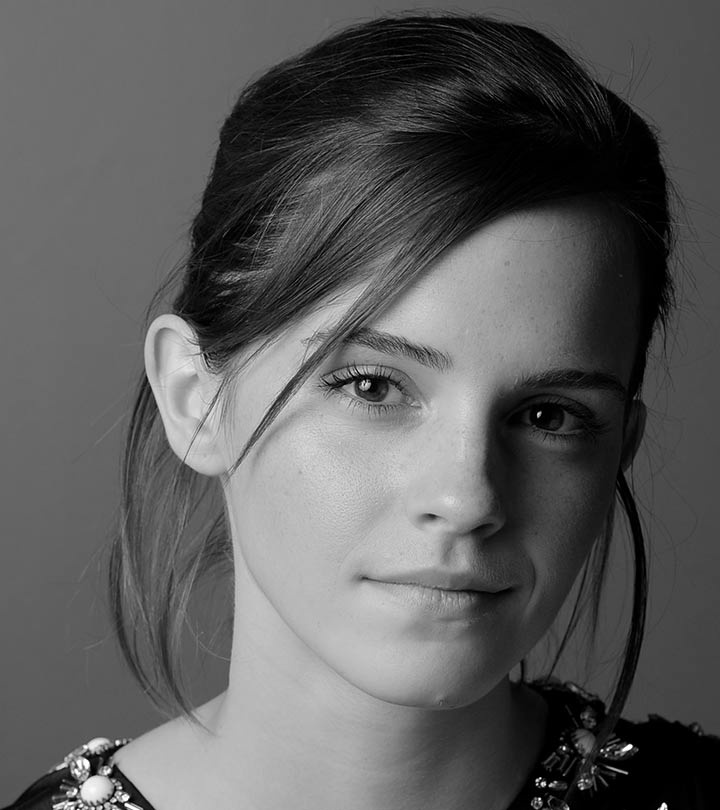
\includegraphics[width=\textwidth]{resources/emma_original.jpg}
        \caption{Original Image}
    \end{subfigure}
    \hfill
    \begin{subfigure}{0.45\textwidth}
        %\fbox{\rule{0pt}{2in}\rule{2in}{0pt}}
        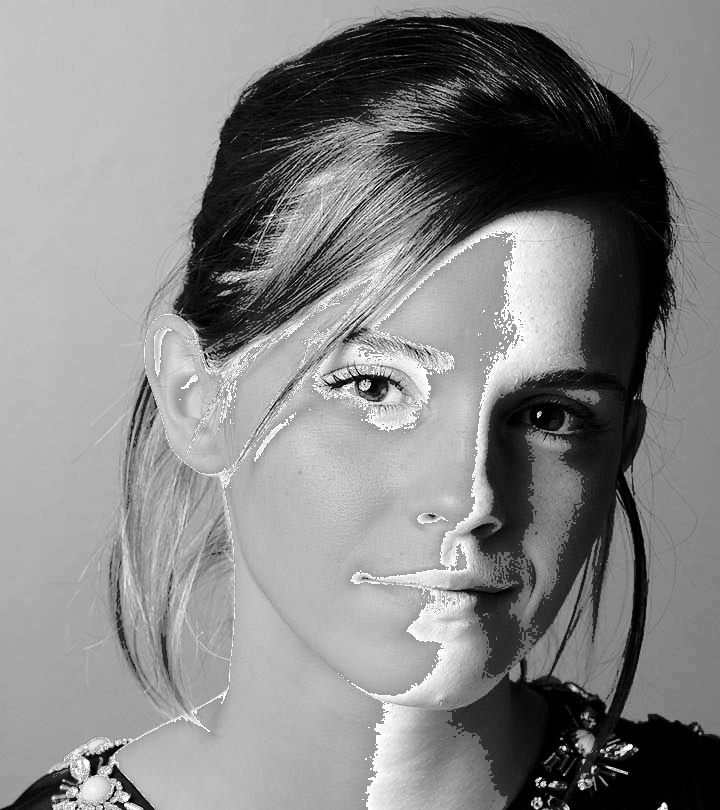
\includegraphics[width=\textwidth]{resources/emma_transformed.jpg}
        \caption{Transformed Image}
    \end{subfigure}
    \caption{Intensity transformation results}
\end{figure}

\subsection{Discussion}
Analysis of the transformation effects and visual changes observed.

\section{Question 2: Brain Image Enhancement}
\subsection{White Matter Accentuation}
\begin{figure}[H]
    \centering
    \begin{subfigure}{0.3\textwidth}
        \fbox{\rule{0pt}{1.5in}\rule{1.5in}{0pt}}
        \caption{Original}
    \end{subfigure}
    \hfill
    \begin{subfigure}{0.3\textwidth}
        \fbox{\rule{0pt}{1.5in}\rule{1.5in}{0pt}}
        \caption{White Matter Enhanced}
    \end{subfigure}
    \hfill
    \begin{subfigure}{0.3\textwidth}
        \fbox{\rule{0pt}{1.5in}\rule{1.5in}{0pt}}
        \caption{Transformation Plot}
    \end{subfigure}
    \caption{White matter enhancement}
\end{figure}

\subsection{Gray Matter Accentuation}
\begin{figure}[H]
    \centering
    \begin{subfigure}{0.3\textwidth}
        \fbox{\rule{0pt}{1.5in}\rule{1.5in}{0pt}}
        \caption{Original}
    \end{subfigure}
    \hfill
    \begin{subfigure}{0.3\textwidth}
        \fbox{\rule{0pt}{1.5in}\rule{1.5in}{0pt}}
        \caption{Gray Matter Enhanced}
    \end{subfigure}
    \hfill
    \begin{subfigure}{0.3\textwidth}
        \fbox{\rule{0pt}{1.5in}\rule{1.5in}{0pt}}
        \caption{Transformation Plot}
    \end{subfigure}
    \caption{Gray matter enhancement}
\end{figure}

\section{Question 3: Gamma Correction}
\subsection{L*a*b* Color Space Conversion}
Explanation of color space conversion and gamma correction application.

\subsection{Gamma Value Selection}
Report the chosen $\gamma$ value and justification.

\subsection{Histogram Analysis}
\begin{figure}[H]
    \centering
    \begin{subfigure}{0.45\textwidth}
        \fbox{\rule{0pt}{1.5in}\rule{2in}{0pt}}
        \caption{Original Histogram}
    \end{subfigure}
    \hfill
    \begin{subfigure}{0.45\textwidth}
        \fbox{\rule{0pt}{1.5in}\rule{2in}{0pt}}
        \caption{Gamma Corrected Histogram}
    \end{subfigure}
    \caption{Histogram comparison before and after gamma correction}
\end{figure}

\section{Question 4: Vibrance Enhancement}
\subsection{HSV Decomposition}
\begin{figure}[H]
    \centering
    \begin{subfigure}{0.3\textwidth}
        \fbox{\rule{0pt}{1.5in}\rule{1.5in}{0pt}}
        \caption{Hue}
    \end{subfigure}
    \hfill
    \begin{subfigure}{0.3\textwidth}
        \fbox{\rule{0pt}{1.5in}\rule{1.5in}{0pt}}
        \caption{Saturation}
    \end{subfigure}
    \hfill
    \begin{subfigure}{0.3\textwidth}
        \fbox{\rule{0pt}{1.5in}\rule{1.5in}{0pt}}
        \caption{Value}
    \end{subfigure}
    \caption{HSV plane decomposition}
\end{figure}

\subsection{Vibrance Transformation}
Implementation of the given formula:
\[
f(x) = \min\left(\mu x + a \times 128 e^{-\frac{(x-128)^2}{2\sigma^2}}, 255\right)
\]
where $a \in [0,1]$ and $\sigma = 70$.

\subsection{Parameter Selection}
Report the chosen value of parameter $a$ and justification.

\subsection{Results Comparison}
Show original, enhanced, and transformation curve.

\section{Question 5: Histogram Equalization}
\subsection{Custom Implementation}
\textbf{Python Implementation:}
\begin{lstlisting}[style=pythonstyle]
def histogram_equalization(image):
    # Your custom Python implementation
    hist, bins = np.histogram(image.flatten(), 256, [0, 256])
    cdf = hist.cumsum()
    # Normalize and apply transformation
    pass
\end{lstlisting}

\textbf{C++ Implementation (Alternative):}
\begin{lstlisting}[style=cppstyle]
Mat histogramEqualization(const Mat& image) {
    Mat result;
    // Calculate histogram
    vector<int> hist(256, 0);
    for (int i = 0; i < image.rows; i++) {
        for (int j = 0; j < image.cols; j++) {
            hist[image.at<uchar>(i, j)]++;
        }
    }
    // Your custom C++ implementation
    return result;
}
\end{lstlisting}

\subsection{Results and Analysis}
Compare histograms before and after equalization.

\section{Question 6: Foreground Histogram Equalization}
\subsection{HSV Analysis and Masking}
Process of selecting appropriate plane for thresholding.

\subsection{Foreground Extraction}
Use of \texttt{cv.bitwise\_and} for foreground isolation.

\subsection{Selective Histogram Equalization}
Application of histogram equalization only to foreground.

\subsection{Results}
Show all intermediate steps and final result.

\section{Question 7: Sobel Filtering}
\subsection{Method 1: Using filter2D}
Implementation using existing OpenCV functions.

\textbf{Python:}
\begin{lstlisting}[style=pythonstyle]
# Sobel kernels
sobel_x = np.array([[-1, 0, 1], [-2, 0, 2], [-1, 0, 1]], dtype=np.float32)
sobel_y = np.array([[-1, -2, -1], [0, 0, 0], [1, 2, 1]], dtype=np.float32)

grad_x = cv2.filter2D(image, cv2.CV_32F, sobel_x)
grad_y = cv2.filter2D(image, cv2.CV_32F, sobel_y)
\end{lstlisting}

\textbf{C++:}
\begin{lstlisting}[style=cppstyle]
// Sobel kernels
Mat sobel_x = (Mat_<float>(3,3) << -1, 0, 1, -2, 0, 2, -1, 0, 1);
Mat sobel_y = (Mat_<float>(3,3) << -1, -2, -1, 0, 0, 0, 1, 2, 1);

Mat grad_x, grad_y;
filter2D(image, grad_x, CV_32F, sobel_x);
filter2D(image, grad_y, CV_32F, sobel_y);
\end{lstlisting}

\subsection{Method 2: Custom Implementation}
Your own Sobel filter implementation.

\subsection{Method 3: Separable Filters}
Using the property:
\[
\begin{bmatrix} 1 & 0 & -1 \\ 2 & 0 & -2 \\ 1 & 0 & -1 \end{bmatrix} 
= \begin{bmatrix} 1 \\ 2 \\ 1 \end{bmatrix} * \begin{bmatrix} 1 & 0 & -1 \end{bmatrix}
\]

\subsection{Results Comparison}
Compare outputs from all three methods.

\section{Question 8: Image Zooming}
\subsection{Interpolation Methods}
Implementation of both nearest-neighbor and bilinear interpolation.

\begin{lstlisting}
def zoom_image(image, scale_factor, method='bilinear'):
    # Your implementation
    pass
\end{lstlisting}

\subsection{Performance Evaluation}
Normalized Sum of Squared Differences (SSD) calculations:
\[
\text{Normalized SSD} = \frac{\sum_{i,j}(I_1(i,j) - I_2(i,j))^2}{\sum_{i,j}I_1(i,j)^2}
\]

\subsection{Results Analysis}
Compare visual quality and SSD values.

\section{References}
\begin{itemize}
    \item OpenCV Documentation: \url{https://opencv.org/}
    \item Gonzalez, R. C., \& Woods, R. E. (2018). \textit{Digital Image Processing} (4th ed.). Pearson.
    \item Stack Overflow and OpenCV forums for implementation help.
\end{itemize}


%%%%%%%%%%%%%%%%%%%%%%%%%%%%%%%%%%%%%%%%%%%%%%%%%%%%%%%%%%
% References
%%%%%%%%%%%%%%%%%%%%%%%%%%%%%%%%%%%%%%%%%%%%%%%%%%%%%%%%%%

% \newpage
% \addcontentsline{toc}{section}{References}
% \bibliographystyle{IEEEtran}
% \bibliography{references}

\end{document}

























